%% LaTeX-Beamer template for KIT design
%% by Erik Burger, Christian Hammer
%% title picture by Klaus Krogmann
%%
%% version 2.0
%%
%% mostly compatible to KIT corporate design v2.0
%% http://intranet.kit.edu/gestaltungsrichtlinien.php
%%
%% Problems, bugs and comments to
%% burger@kit.edu

\documentclass[18pt]{beamer}
\usetheme{kit}

%% TITLE PICTURE

% if a custom picture is to be used on the title page, copy it into the 'logos'
% directory, in the line below, replace 'mypicture' with the 
% filename (without extension) and uncomment the following line
% (picture proportions: 63 : 20, *.eps format if you use latex+dvips+ps2pdf,
% *.jpg/*.png/*.pdf if you use pdflatex)

%\titleimage{mypicture}

%% TITLE LOGO

% for a custom logo on the front page, copy your file into the 'logos'
% directory, insert the filename in the line below and uncomment it

%\titlelogo{mylogo}

% (*.eps format if you use latex+dvips+ps2pdf,
% *.jpg/*.png/*.pdf if you use pdflatex)

%% BIBTEX ICON/KEY

% if you want to see BibTeX keys in the references view instead of the symbol,
% uncomment the following line
% \usebibitemtemplate{\insertbiblabel}

% the presentation starts here

\title[Short title]{Tutorium 01: Projektplanung }
\subtitle{Softwaretechnik im SS 2011, Tutorien 4 + X + Y}
\author{Jürgen Walter}

\institute{Chair for Software Design and Quality}

\begin{document}

% change the following line to "ngerman" for German style date and logos
% change the following line to "english" for English style date and logos
\selectlanguage{ngerman}

%title page
\begin{frame}
\titlepage
\end{frame}

\section{Organisatorisches}

\subsection{Vorstellung}
\frame{
\frametitle{Wer bin ich?}
\begin{itemize}
\item Jürgen Walter
\pause
\item 8tes Semester Informatik
\pause
\item juergen.walter.halle@gmail.com
\item uxccx@student.kit.edu
\pause
\item Partnerturoren Christian Juelg und Daniel Deckers
\item \dots
\end{itemize}
}

%table of contents
\frame{
\frametitle{Was machen wir heute?}
\tableofcontents
}

\subsection{Übungsschein}
\frame{
\frametitle{Übungsschein}
\begin{block}{Der Übungsschein \dots}
\begin{itemize}
\pause
\item ist keine Vorraussetzung zur Klausur, aber Vorraussetzung für Modul!
\pause
\item hat 6 Übungsblätter mit  insgesammt 150 Punkten
\pause
\item ist mit 50 Prozent aus Übungsblättern und Programmmieraufgaben bestanden 
\end{itemize}
\end{block}
}


\section{Altes Übungsblatt und Wiederholungen}

\subsection{Altes Übungsblatt}
\frame {
\frametitle{Altes Übungsblatt}
\begin{block}{Aufgabe 1: Mailingliste}
\begin{itemize}
\item ...
\end{itemize}
\end{block}


\begin{block}{Aufgabe 2: Lastenheft}
\begin{enumerate}
\item Zielbestimmung
\item Produkteinsatz
\item Funktionale Anforderungen
\item Produktdaten
\item Nichtfunktionale Anforderungen
\item Systemmodelle
\begin{itemize}
	\item Szenarien
	\item Anwendungsfälle
\end{itemize}
\item Glossar (Begriffslexikon zur Beschreibung des Produktes)
\end{enumerate}
\end{block}
}

\frame {
\begin{block}{Aufgabe 3 Durchführbarkeitsuntersuchung} 
\begin{itemize}
\item ...
\end{itemize}

\end{block}
\begin{block}{Aufgabe 4 Hans Olo}
\begin{itemize}
\item \textbf{Benutzt Checkstyle!}
\end{itemize}
\end{block}

\begin{block}{Aufgabe 5 Vorbereitung der Programmieraufgabe}
\begin{itemize}
\item ...
\end{itemize}
\end{block}
}

\subsection{Zum Aufwärmen ...}
\frame {
\frametitle{Wahr oder falsch?}
\begin{itemize}
	\color<2-7>[rgb]{0,1,0}
	\item In der Planungsphase wird die softwaretechnische Realisierbarkeit eines Produktes untersucht
	\color[rgb]{0,0,0}
	\pause
	\color<3-7>[rgb]{1,0,0}
	\item Ein Pflichtenheft beschreibt die Eigenschaften, die das Produkt aus der Sicht des Kunden erfüllen soll
	\color[rgb]{0,0,0}
	\pause
	\color<4-7>[rgb]{0,1,0}
	\item In einem UML-Anwendungsfalldiagramm werden typische Interaktionen des Benutzers mit dem System modelliert
	\color[rgb]{0,0,0}
	\pause
	\color<5-7>[rgb]{1,0,0}
	\item Das Lastenheft ist eine Verfeinerung des Pflichtenheftes
	\color[rgb]{0,0,0}
	\pause
	\color<6-7>[rgb]{1,0,0}
	\item Im Pflichtenheft steht beschrieben, wie etwas zu implementieren ist. Es werden z.B. Algorithmen und Datenstrukturen beschrieben
	\color[rgb]{0,0,0}
\end{itemize}
}


\subsection{Werkzeuge}

\frame{
\frametitle{Versionsverwaltungen}

\begin{block}{Subversion}
\begin{itemize}
\item von der Vorlesung unterstützte Versionsverwaltung
\item Windows: Tortoise SVN
\item Linux: Shell oder Tortoise SVN
\item Mac: Shell
\end{itemize}
\end{block}
\pause

\begin{block}{Git}
\begin{itemize}
\item Werkzeug des Tutors ;-)
\end{itemize}
\end{block}
}

\frame {
\frametitle{Klausuraufgabe 2009}
\begin{block}{Aufgabe}
Erklären Sie die beiden Begriffe „Striktes Ausbuchen“ und „Optimistisches Ausbuchen“ im Kontext einer Konfigurationsverwaltung. Nennen Sie jeweils einen Vor- sowie einen Nachteil. (4P)
\end{block}

Striktes Ausbuchen
\visible <2-> {
\begin{itemize}
\item Nur eine Ausbuchung gleichzeitig ist erlaubt 
\item Ausbucher hat exklusives Änderungsrecht 
\item Vorteil: kein Verschmelzungsaufwand beim Zurückschreiben 
\item Nachteil: immer nur einer kann eine Version ändern
\end{itemize}
}
Optimistisches Ausbuchen 
\visible<3-> {
\begin{itemize}
\item Mehrere Ausbuchungen gleichzeitig erlaubt 
\item Mehrere Entwickler Arbeiten an der gleichen Programmversion 
\item Vorteil: Mehrere Entwickler können eine Version ändern 
\item Nachteil: Aufwand beim Zusammenführen der Versionen (der Schnellere gewinnt)
\end{itemize}
}
}


\frame{
\frametitle{Checkstyle}
\begin{alertblock}{Das geht besser \dots}
\begin{itemize}
\item Keiner von euch ist ohne Checkstyle Fehler
\end{itemize}
\end{alertblock}
}



\subsection{Lastenheft}

\frame{
\frametitle{Lastenheft}
\begin{itemize}
\item enthält die Hauptanforderungen an das Produkt (user requirements)
\item formuliert mit natürlicher Sprache, evtl. Diagramme
\item dient der Kommunikation mit dem Kunden und der Projektplanung
\end{itemize}
}

\frame{
\frametitle{Klassendiagramm}
Hier könnte man dann etwas allgemeines zu Klassendiagrammen sagen

Ist Aufgabe 1 vom Übungsblatt 2
}

\frame {
\frametitle{Klassendiagramm Aufgabe}
\begin{block} {Szenario}  
In einer Formel 1-Saison gibt es 12 Teams. Die Saison hat 19 Rennen und an jedem Rennen nehmen
die Teams mit jeweils 2 Fahrzeugen teil. Während der Saison können Teams ausscheiden und von
nachrückenden Teams ersetzt werden. Es kann aber niemals in dieser Saison weniger als eins oder
mehr als 12 Teams geben. Zu den öffentlichen Eigenschaften eines Fahrzeugs gehört der Team-
Name, der Name des Chassis, die Motorbezeichnung sowie Startnummer und der Fahrer. Die Startnummer
ist eindeutig. Die geheimen Eigenschaften eines Fahrzeugs sind die Größe des Tanks und
die Dicke der Bodenplatte. In dieser Saison gibt es verschiedene Motoren, die von den zwölf Teams
in ihren beiden Fahrzeugen verbaut sind.
\end{block}

Verwenden Sie die aus der Vorlesung bekannten Vorgehensweisen zur Objektmodellierung und erstellen Sie
ein Klassendiagramm. Modellieren Sie dabei Klassen, Attribute, Assoziationen und Multiplizitäten.

}

\subsection{Pflichtenheft}

\frame{
\frametitle{Pflichtenheft}
\begin{block}{Gliederungsschema Pflichtenheft}
\begin{itemize}
\item\dots
\end{itemize}
\end{block}
}

\frame{
\frametitle{Musterlösung}
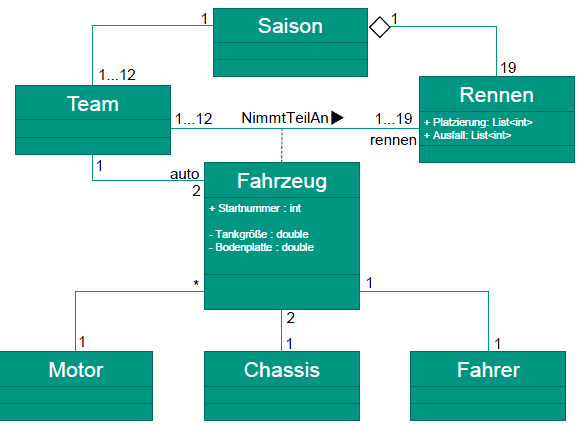
\includegraphics[scale=0.5]{pics/Klassendiagramm.png}

}

\section{Ende}

\frame{
\frametitle{Tipps zum nächsten Übungsblatt}

\begin{block}{Aufgabe 1}
\begin{itemize}
\item Bla bla
\item Bla bla
\end{itemize}
\end{block}

\begin{block}{Aufgabe 2}
\begin{itemize}
\item Bla bla
\item Bla bla
\end{itemize}
\end{block}

\begin{block}{Aufgabe 3}
\begin{itemize}
\item Bla bla
\item Bla bla
\end{itemize}
\end{block}


}


\frame{
\frametitle{Bis zum nächsten Mal}
\begin{center}
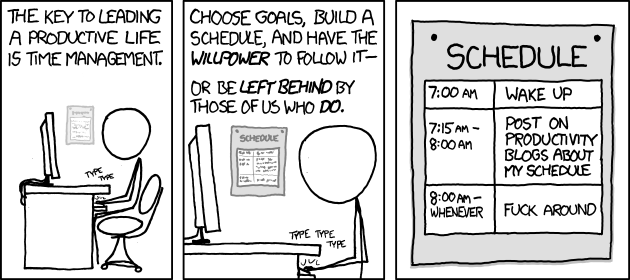
\includegraphics[width=1\textwidth]{pics/time_management}
\end{center}

}


\end{document}
